\documentclass[aps,prl,preprint,notitlepage]{revtex4-1}

\usepackage{amsmath}
\usepackage{graphicx}

\renewcommand{\vec}[1]{\boldsymbol{#1}}

\begin{document}

\title{Rotation and acceleration in vectorial solenoidal wave packets}

\author{Argha Mondal}
\affiliation{Department of Physics, New York University,
New York, NY 10003}

\maketitle

In \cite{mondal18a}, we showed that
superpositions of scalar Bessel wave functions
may appear to correspond to classical trajectories
undergoing uniform circular motion.
The analysis in \cite{mondal18a} reveals that these
states are not accelerating after all, and indeed are not
even rotating.
Instead, the expectation value of the two-dimensional
position travels with constant speed along a straight line
in agreement with Ehrenfest's theorem.
The discrepancy between these states' apparent rotation
and their actual translation is due to the small amount
of diffraction that arises inevitably for Bessel modes
of finite spatial extent.

\begin{figure*}
\centering
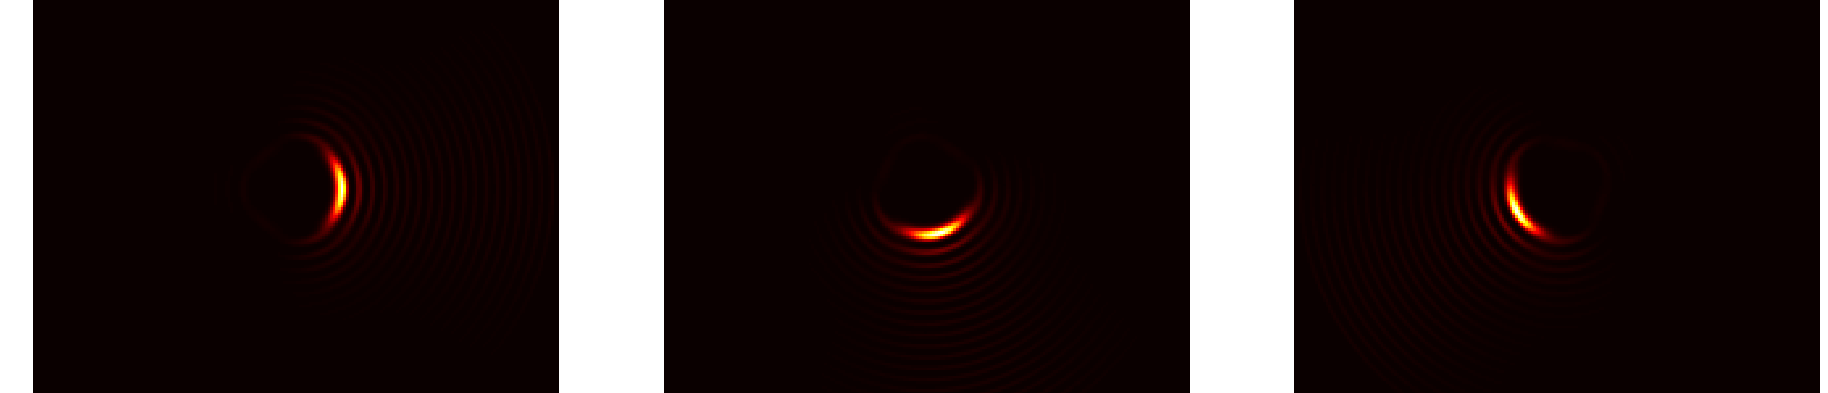
\includegraphics[width=0.75\textwidth]{pic2}
\caption{If $\Delta n = 1$ and $n = 10$ we have the dynamics as shown above.}
\end{figure*}

These observations raise questions about the behavior of
analogous solenoidal states of light.
Whereas a scalar wave function is appropriate for
a quantum mechanical particle, it only describes a
beam of light in the paraxial approximation.
What differences, if any, arise when account is taken
of the vector nature of light?

To address this question, we consider the time evolution of
a solenoidal mode created from vector Bessel beams.
For simplicity, we consider radially-polarized TE
modes as illustrative examples.
A radially-polarized Bessel mode whose amplitude
vanishes at radial distance $r = R$ from the optical
axis may be described
with the vector potential
\begin{equation}
  \vec{A}_{n,\nu}(\vec{r},t) 
  = 
  A_{n,\nu} J_{n}\!\left( \sin \alpha_{n,\nu} \, k r \right)
  e^{in\phi} e^{i\cos\alpha_{n,\nu} \, kz} e^{- i \omega t},
\end{equation}
where $k = \omega/c$ is the wave number of light at
frequency $\omega$, $J_n(x)$ is the $n$-th order
Bessel function of the first kind and $A_{n,\nu}$ is
the amplitude.
The convergence angle $\alpha_{n\nu}$ satisfies
the boundary condition at $r = R$
if $kR \sin\alpha_{n,\nu} = j_{n,\nu}$,
where $j_{n,\nu}$ is the $\nu$-th zero of $J_n(x)$.

A solenoidal mode of the kind described in \cite{mondal18a}
is created as a superposition
\begin{equation}
  \label{eq:solenoid}
  \vec{A}(\vec{r},t)
  =
  \frac{1}{\sqrt{2}} \left[
    \vec{A}_{n,\nu}(\vec{r},t) +
    \vec{A}_{n',\nu'}(\vec{r},t)
  \right] .
\end{equation}
We use the following equation to calculate the electric field:
\begin{equation}
\vec{E} = ik\left[\vec{A} + \frac{1}{k^2}\bigtriangledown (\bigtriangledown \cdot \vec{A})\right]
\end{equation}
In cylindrical coordinate:
\begin{equation}
\vec{E_r} = \frac{i}{\sqrt{2}k}\left[ C_{n,\nu}(J_{n-1}(\varrho) 
- J_{n+1}(\varrho)) e^{in\phi}e^{i(kz\cos \alpha _n - \omega t)} +
C_{n\prime,\nu \prime}(J_{n\prime-1}(\varrho) - J_{n\prime+1}(\varrho))
e^{in\prime\phi}e^{i(kz\cos \alpha _{n\prime} - \omega t)}\right] \hat{r}
\end{equation}
,where $C_{n,\nu} = A_{n,\nu}ik\cos \alpha _{n}\frac{j_{n,\nu}}{2R}$, 
$\varrho = j_{n,\nu}\frac{r}{R}$, and $\alpha _{n} = \arccos \left( 
\sqrt{1-\frac{j_{n,\nu}^2}{k^2 R^2}}\right)$
\begin{equation}
\vec{E_{\phi}} = -\frac{i}{\sqrt{2}r}\left[ A_{n,\nu}n\cos \alpha _{n} 
J_{n}(\varrho)e^{in\phi}e^{i(kz\cos \alpha _{n} - \omega t)} + 
A_{n\prime,\nu \prime}n\prime \cos \alpha _{n\prime} J_{n\prime}(\varrho)
e^{in\prime \phi}e^{i(kz\cos \alpha _{n\prime} - \omega t)}\right] \hat{\phi}
\end{equation}
\begin{equation}
\vec{E_{z}} = \frac{ik}{\sqrt{2}}\left[ A_{n,\nu}\sin ^{2}\alpha _{n} 
J_{n}(\varrho)e^{in\phi}e^{i(kz\cos \alpha _{n} - \omega t)} + 
A_{n\prime,\nu \prime}\sin ^{2}\alpha _{n \prime} J_{n \prime}(\varrho)
e^{in\prime \phi}e^{i(kz\cos \alpha _{n\prime} - \omega t)} \right] \hat{z}
\end{equation}
Say $\Delta n = |n - n\prime|$. If $\Delta n = 1$ and $n = 10$ we have the following dynamics of $\rho(\vec{r},t) = |E_r(\vec{r})|^2$,


\bibliography{abbreviations,grier}

\end{document}